\chapter{Experimental Setup}
\label{Chap:experimental}

In this chapter we introduce the experimental setup used for our experiments.
We start by presenting the design of our implementation of a qubit: the Transmon.
Then we will show how the qubit is driven for our purposes, in particular how to perform readout and 2-qubit gates.

Finally we put everything together and present the chip used for quantum entangling and photon emission.

\section{The Qubit}
\label{sec:qubit}

The basic idea behind the implementation of a device for quantum information is realizing a 2-level quantum system.
In the Quantum Device Lab we use superconducting circuits.

\subsection{Quantum LC resonator}

To introduce the implementation of the qubit utilized in our laboratory, we begin by presenting a simplified model: the quantum LC resonator \cite{LC_resonator}.
\begin{figure}
    \begin{minipage}[b]{0.5\linewidth}
      \centering
        

\tikzset{every picture/.style={line width=0.75pt}} %set default line width to 0.75pt        

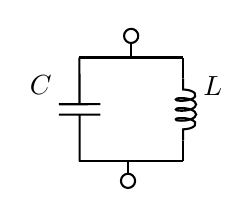
\begin{tikzpicture}[x=0.75pt,y=0.75pt,yscale=-1,xscale=1]
%uncomment if require: \path (0,97); %set diagram left start at 0, and has height of 97

%Shape: Capacitor [id:dp4670171494463129] 
\draw  [line width=0.75]  (50,23.83) -- (50.05,46.33) (60.07,51.31) -- (40.07,51.36) (60.05,46.31) -- (40.05,46.36) (50.07,51.33) -- (50.12,73.83) ;
%Straight Lines [id:da7530368359567341] 
\draw [line width=0.75]    (50,23.83) -- (100,23.83) ;
%Straight Lines [id:da37073903294106214] 
\draw [line width=0.75]    (50,73.83) -- (100,73.83) ;
%Straight Lines [id:da6760299644418128] 
\draw [line width=0.75]    (100,23.83) -- (100,33.83) ;
%Straight Lines [id:da16342394128001536] 
\draw [line width=0.75]    (100,63.83) -- (100,73.83) ;
%Straight Lines [id:da10569605743197075] 
\draw [line width=0.75]    (73.42,79.83) -- (73.42,73.83) ;
%Shape: Circle [id:dp3114709006095975] 
\draw  [line width=0.75]  (70,83.25) .. controls (70,81.36) and (71.53,79.83) .. (73.42,79.83) .. controls (75.3,79.83) and (76.83,81.36) .. (76.83,83.25) .. controls (76.83,85.14) and (75.3,86.67) .. (73.42,86.67) .. controls (71.53,86.67) and (70,85.14) .. (70,83.25) -- cycle ;
%Straight Lines [id:da44379321850243414] 
\draw [line width=0.75]    (75,16.83) -- (75,23.83) ;
%Shape: Circle [id:dp37786908957841614] 
\draw  [line width=0.75]  (78.33,13.33) .. controls (78.38,15.22) and (76.89,16.78) .. (75,16.83) .. controls (73.11,16.88) and (71.55,15.39) .. (71.5,13.5) .. controls (71.45,11.62) and (72.94,10.05) .. (74.83,10) .. controls (76.71,9.95) and (78.28,11.44) .. (78.33,13.33) -- cycle ;
%Shape: Inductor (Air Core) [id:dp009772684946594334] 
\draw   (100,33.83) -- (100,39.23) .. controls (102.63,39.31) and (104.87,40.06) .. (105.66,41.12) .. controls (106.44,42.18) and (105.61,43.34) .. (103.55,44.03) .. controls (101.95,44.57) and (99.88,44.79) .. (97.87,44.63) .. controls (97.08,44.63) and (96.45,44.36) .. (96.45,44.03) .. controls (96.45,43.7) and (97.08,43.43) .. (97.87,43.43) .. controls (99.88,43.28) and (101.95,43.5) .. (103.55,44.03) .. controls (105.26,44.66) and (106.23,45.52) .. (106.23,46.43) .. controls (106.23,47.34) and (105.26,48.21) .. (103.55,48.83) .. controls (101.95,49.37) and (99.88,49.59) .. (97.87,49.43) .. controls (97.08,49.43) and (96.45,49.16) .. (96.45,48.83) .. controls (96.45,48.5) and (97.08,48.23) .. (97.87,48.23) .. controls (99.88,48.08) and (101.95,48.3) .. (103.55,48.83) .. controls (105.26,49.46) and (106.23,50.32) .. (106.23,51.23) .. controls (106.23,52.14) and (105.26,53.01) .. (103.55,53.63) .. controls (101.95,54.17) and (99.88,54.39) .. (97.87,54.23) .. controls (97.08,54.23) and (96.45,53.96) .. (96.45,53.63) .. controls (96.45,53.3) and (97.08,53.03) .. (97.87,53.03) .. controls (99.88,52.88) and (101.95,53.1) .. (103.55,53.63) .. controls (105.61,54.33) and (106.44,55.48) .. (105.66,56.54) .. controls (104.87,57.61) and (102.63,58.35) .. (100,58.43) -- (100,63.83) ;

% Text Node
\draw (108.23,43.43) node [anchor=south west] [inner sep=0.75pt]   [align=left] {$\displaystyle L$};
% Text Node
\draw (38.05,43.36) node [anchor=south east] [inner sep=0.75pt]   [align=left] {$\displaystyle C$};


\end{tikzpicture}
        \vspace{-0.7cm}
        \caption{Circuit diagram of LC resonator}
        \label{fig:LC}
    \end{minipage}
    \hfill
    \begin{minipage}[b]{0.45\linewidth}
      \centering
      

\tikzset{every picture/.style={line width=0.75pt}} %set default line width to 0.75pt        

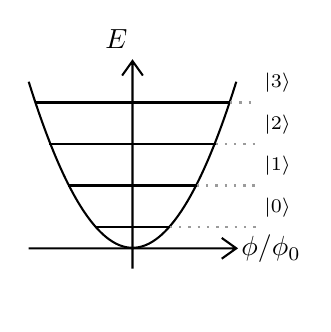
\begin{tikzpicture}[x=0.75pt,y=0.75pt,yscale=-1,xscale=1]
%uncomment if require: \path (0,200); %set diagram left start at 0, and has height of 200

%Shape: Parabola [id:dp37890511708987873] 
\draw   (60,70) .. controls (93.33,176.67) and (126.67,176.67) .. (160,70) ;
%Shape: Axis 2D [id:dp3773695523891737] 
\draw  (60,150.25) -- (160,150.25)(110,60) -- (110,160) (153,145.25) -- (160,150.25) -- (153,155.25) (105,67) -- (110,60) -- (115,67)  ;
%Straight Lines [id:da3077075366408746] 
\draw    (92,140) -- (128,140) ;
%Straight Lines [id:da2626121978197561] 
\draw    (79,120) -- (141,120) ;
%Straight Lines [id:da8498237157026597] 
\draw    (70,100) -- (150,100) ;
%Straight Lines [id:da16494940971997396] 
\draw    (63,80) -- (157,80) ;
%Straight Lines [id:da15643784358380952] 
\draw [color={rgb, 255:red, 155; green, 155; blue, 155 }  ,draw opacity=1 ] [dash pattern={on 0.84pt off 2.51pt}]  (128,140) -- (170,140) ;
%Straight Lines [id:da7225933392434986] 
\draw [color={rgb, 255:red, 155; green, 155; blue, 155 }  ,draw opacity=1 ] [dash pattern={on 0.84pt off 2.51pt}]  (141,120) -- (170,120) ;
%Straight Lines [id:da6235512774693245] 
\draw [color={rgb, 255:red, 155; green, 155; blue, 155 }  ,draw opacity=1 ] [dash pattern={on 0.84pt off 2.51pt}]  (150,100) -- (170,100) ;
%Straight Lines [id:da04257430271569573] 
\draw [color={rgb, 255:red, 155; green, 155; blue, 155 }  ,draw opacity=1 ] [dash pattern={on 0.84pt off 2.51pt}]  (157,80) -- (170,80) ;

% Text Node
\draw (109,49.5) node [anchor=east] [inner sep=0.75pt]   [align=left] {$\displaystyle E$};
% Text Node
\draw (161,142.4) node [anchor=north west][inner sep=0.75pt]    {$\phi /\phi _{0}$};
% Text Node
\draw (172,136.6) node [anchor=south west] [inner sep=0.75pt]  [font=\scriptsize]  {$| 0\rangle $};
% Text Node
\draw (172,116.6) node [anchor=south west] [inner sep=0.75pt]  [font=\scriptsize]  {$| 1\rangle $};
% Text Node
\draw (172,96.6) node [anchor=south west] [inner sep=0.75pt]  [font=\scriptsize]  {$| 2\rangle $};
% Text Node
\draw (172,76.6) node [anchor=south west] [inner sep=0.75pt]  [font=\scriptsize]  {$| 3\rangle $};


\end{tikzpicture}
      \vspace{-1.5cm}
      \caption{Energy spectrum of LC resonator}
      \label{fig:Energy_spectrum}
    \end{minipage}
  \end{figure}
The circuit diagram is illustrated in \cref{fig:LC}, depicting a system that emulates the behavior of a quantum oscillator.
In classical physics, the Hamiltonian for a harmonic oscillator is expressed as follows:
\begin{equation}
    H = \frac{\phi^2}{2L} + \frac{Q^2}{2C},
\end{equation}
where $\phi$ represents the flux in the inductor, and $Q$ denotes the charge on the capacitor.

Quantizing this classical Hamiltonian involves replacing $\phi$ and $Q$ with the flux operator ($\hat{\phi}$) and charge operator ($\hat{Q}$), respectively.
The resulting quantum Hamiltonian, expressed in second quantization form, is given by:
\begin{equation}
    \hat{H} = \frac{\hat{\phi}^2}{2L} + \frac{\hat{Q}^2}{2C} = \hbar \omega \left(\hat{a}^\dagger \hat{a} + \frac{1}{2}\right),
\end{equation}
where $\omega = 1/\sqrt{LC}$ is the resonance frequency of the circuit.
The operators $\hat{a}^\dagger$ and $\hat{a}$ correspond to the creation and annihilation operators of excitations, respectively. 
In this scenario, the excitations represent the difference in the number of charges between the two plates of the capacitor.
Utilizing this quantum description of the LC circuit, we obtain the energy spectrum illustrated in \cref{fig:Energy_spectrum} ($\phi_0 = h/2e$ is the flux quantum) .
The quantization of energy levels in relation to the magnetic flux $\phi$ is clearly evident in the figure.

\subsection{The transmon resonator}

The issue of energy level harmonicity poses a challenge when aiming to construct a quantum processor. 
In this context, determining the specific transitions being driven becomes uncertain, as the energy differences between consecutive levels remain identical.
To address this, we introduce non-linearity into our circuit through the incorporation of the Josephson junction \cite{JOSEPHSON}.

Josephson demonstrated that a current without dissipation could flow between two superconducting electrodes when separated by a thin insulating barrier. Specifically, he established that this supercurrent is determined by
\begin{equation}
    I = I_c \sin(\varphi),
\end{equation}
where $I_c$ represents the critical current of the junction, and $\varphi$ denotes the phase difference between the superconducting condensates on each side of the junction.
\begin{figure}
    \begin{minipage}[b]{0.5\linewidth}
      \centering
        

\tikzset{every picture/.style={line width=0.75pt}} %set default line width to 0.75pt        

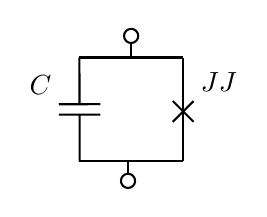
\begin{tikzpicture}[x=0.75pt,y=0.75pt,yscale=-1,xscale=1]
%uncomment if require: \path (0,97); %set diagram left start at 0, and has height of 97

%Shape: Capacitor [id:dp8072216489364277] 
\draw  [line width=0.75]  (60,23.83) -- (60.05,46.33) (70.07,51.31) -- (50.07,51.36) (70.05,46.31) -- (50.05,46.36) (60.07,51.33) -- (60.12,73.83) ;
%Straight Lines [id:da183774352314787] 
\draw [line width=0.75]    (105,54.83) -- (115,44.83) ;
%Straight Lines [id:da1896922658483372] 
\draw [line width=0.75]    (105,44.83) -- (115,54.83) ;

%Straight Lines [id:da33699096520016336] 
\draw [line width=0.75]    (60,23.83) -- (110,23.83) ;
%Straight Lines [id:da6915014186556621] 
\draw [line width=0.75]    (60,73.83) -- (110,73.83) ;
%Straight Lines [id:da36159548727595725] 
\draw [line width=0.75]    (83.42,79.83) -- (83.42,73.83) ;
%Shape: Circle [id:dp8015144235751568] 
\draw  [line width=0.75]  (80,83.25) .. controls (80,81.36) and (81.53,79.83) .. (83.42,79.83) .. controls (85.3,79.83) and (86.83,81.36) .. (86.83,83.25) .. controls (86.83,85.14) and (85.3,86.67) .. (83.42,86.67) .. controls (81.53,86.67) and (80,85.14) .. (80,83.25) -- cycle ;
%Straight Lines [id:da3714464315940995] 
\draw [line width=0.75]    (85,16.83) -- (85,23.83) ;
%Shape: Circle [id:dp25364190410803145] 
\draw  [line width=0.75]  (88.33,13.33) .. controls (88.38,15.22) and (86.89,16.78) .. (85,16.83) .. controls (83.11,16.88) and (81.55,15.39) .. (81.5,13.5) .. controls (81.45,11.62) and (82.94,10.05) .. (84.83,10) .. controls (86.71,9.95) and (88.28,11.44) .. (88.33,13.33) -- cycle ;
%Straight Lines [id:da8131700138845456] 
\draw    (110,23.83) -- (110,73.83) ;

% Text Node
\draw (48.05,43.36) node [anchor=south east] [inner sep=0.75pt]   [align=left] {$\displaystyle C$};
% Text Node
\draw (117,41.83) node [anchor=south west] [inner sep=0.75pt]   [align=left] {$\displaystyle JJ$};


\end{tikzpicture}
        \vspace{-0.8cm}
        \caption{Circuit diagram of a transmon resonator}
        \label{fig:JJ_circuit}
    \end{minipage}
    \hfill
    \begin{minipage}[b]{0.45\linewidth}
      \centering
      

\tikzset{every picture/.style={line width=0.75pt}} %set default line width to 0.75pt        

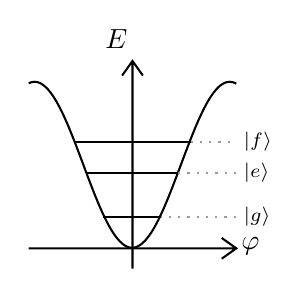
\begin{tikzpicture}[x=0.75pt,y=0.75pt,yscale=-1,xscale=1]
%uncomment if require: \path (0,200); %set diagram left start at 0, and has height of 200

%Straight Lines [id:da03495800698048135] 
\draw [color={rgb, 255:red, 155; green, 155; blue, 155 }  ,draw opacity=1 ] [dash pattern={on 0.84pt off 2.51pt}]  (123,135) -- (160,135) ;
%Shape: Axis 2D [id:dp2373273044965445] 
\draw  (60,150.25) -- (160,150.25)(110,60) -- (110,160) (153,145.25) -- (160,150.25) -- (153,155.25) (105,67) -- (110,60) -- (115,67)  ;
%Shape: Wave [id:dp12933752750229321] 
\draw   (60,70.71) .. controls (60.93,70.25) and (61.87,70) .. (62.82,70) .. controls (71.32,70) and (78.66,89.51) .. (86.32,110) .. controls (93.98,130.49) and (101.32,150) .. (109.82,150) .. controls (118.32,150) and (125.66,130.49) .. (133.32,110) .. controls (140.98,89.51) and (148.32,70) .. (156.82,70) .. controls (157.9,70) and (158.96,70.31) .. (160,70.9) ;
%Straight Lines [id:da530045401686506] 
\draw    (96,135) -- (123,135) ;
%Straight Lines [id:da34934240050097976] 
\draw    (88,114) -- (132,114) ;
%Straight Lines [id:da19311872891258342] 
\draw    (82,99) -- (138,99) ;
%Straight Lines [id:da3065730660397551] 
\draw [color={rgb, 255:red, 155; green, 155; blue, 155 }  ,draw opacity=1 ] [dash pattern={on 0.84pt off 2.51pt}]  (132,114) -- (160,114) ;
%Straight Lines [id:da057644743938617404] 
\draw [color={rgb, 255:red, 155; green, 155; blue, 155 }  ,draw opacity=1 ] [dash pattern={on 0.84pt off 2.51pt}]  (138,99) -- (160,99) ;

% Text Node
\draw (109,49.5) node [anchor=east] [inner sep=0.75pt]   [align=left] {$\displaystyle E$};
% Text Node
\draw (161,143.4) node [anchor=north west][inner sep=0.75pt]    {$\varphi $};
% Text Node
\draw (162,135) node [anchor=west] [inner sep=0.75pt]  [font=\scriptsize]  {$|g\rangle $};
% Text Node
\draw (162,114) node [anchor=west] [inner sep=0.75pt]  [font=\scriptsize]  {$|e\rangle $};
% Text Node
\draw (162,99) node [anchor=west] [inner sep=0.75pt]  [font=\scriptsize]  {$|f\rangle $};


\end{tikzpicture}
      \vspace{-1.2cm}
      \caption{Energy spectrum of transmon resonator}
      \label{fig:Energy_spectrum_JJ}
    \end{minipage}
  \end{figure}

By replacing the inductor of the LC resonator with a Josephson junction (\cref{fig:JJ_circuit}), we achieve the desired anharmonicity of the energy levels.
The resulting potential becomes a cosine potential, leading to non-equidistant energy levels, as illustrated in \cref{fig:Energy_spectrum_JJ}.
To gain a deeper insight into the origin of this anharmonicity, we present the Hamiltonian of the Josephson junction resonator in second quantization formalism:
\begin{equation}
\label{eq:cosina_H}
    \hat{H} = 
    \hbar \omega \hat{a}^\dagger \hat{a} - 
    \frac{E_C}{2}\hat{a}^\dagger\hat{a}^\dagger\hat{a}\hat{a} ,
\end{equation}
where
\begin{equation}
    E_C = \frac{e^2}{2 C_\Sigma}
\end{equation} 
is the charging energy and $C_\Sigma = C_J + C_C$ is the total capacitance.
The Hamiltonian described in \cref{eq:cosina_H} essentially represents an harmonic oscillator incorporating an anharmonicity correction. 
This allows us to address individual energy levels separately.

This arrangement is employed in quantum computation, utilizing the first two energy levels, $\ket{g}$ and $\ket{e}$, for encoding quantum state information. 
Typically, the $\ket{f}$ state is utilized as an auxiliary energy level during the implementation of certain operations.

In our laboratory, the transmon qubit is realized through the Josephson junction resonator under specific conditions known as the \emph{transmon regime} \cite{transmon_regime}.

An advantageous adaptation of the transmon artificial atom is the flux-tunable transmon, in which the single Josephson junction is substituted with two parallel junctions, forming a superconducting quantum interference device (SQUID).
\begin{figure}
    \begin{minipage}[b]{0.5\linewidth}
      \centering
      


\tikzset{every picture/.style={line width=0.75pt}} %set default line width to 0.75pt        

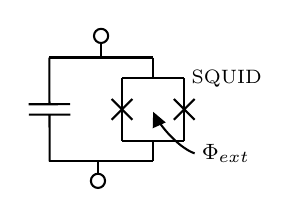
\begin{tikzpicture}[x=0.75pt,y=0.75pt,yscale=-1,xscale=1]
%uncomment if require: \path (0,97); %set diagram left start at 0, and has height of 97

%Shape: Capacitor [id:dp34366919102472526] 
\draw  [line width=0.75]  (20,23.83) -- (20.05,46.33) (30.07,51.31) -- (10.07,51.36) (30.05,46.31) -- (10.05,46.36) (20.07,51.33) -- (20.12,73.83) ;
%Straight Lines [id:da9532858123226031] 
\draw [line width=0.75]    (55,33.83) -- (85,33.83) ;
%Straight Lines [id:da4790035249190253] 
\draw [line width=0.75]    (85,33.83) -- (85,63.83) ;
%Straight Lines [id:da5192559786668693] 
\draw [line width=0.75]    (55,33.83) -- (55,63.83) ;
%Straight Lines [id:da23389027703175358] 
\draw [line width=0.75]    (55,63.83) -- (85,63.83) ;
%Straight Lines [id:da6028752523424945] 
\draw [line width=0.75]    (50,43.83) -- (60,53.83) ;
%Straight Lines [id:da22268293223346158] 
\draw [line width=0.75]    (50,53.83) -- (60,43.83) ;
%Straight Lines [id:da7666685944565205] 
\draw [line width=0.75]    (80,53.83) -- (90,43.83) ;
%Straight Lines [id:da0860971350076063] 
\draw [line width=0.75]    (80,43.83) -- (90,53.83) ;
%Straight Lines [id:da32147396047949894] 
\draw [line width=0.75]    (20,23.83) -- (70,23.83) ;
%Straight Lines [id:da3842851758264739] 
\draw [line width=0.75]    (20,73.83) -- (70,73.83) ;
%Straight Lines [id:da04257544936461244] 
\draw [line width=0.75]    (70,23.83) -- (70,33.83) ;
%Straight Lines [id:da22754146049716317] 
\draw [line width=0.75]    (70,63.83) -- (70,73.83) ;
%Straight Lines [id:da6459112049306985] 
\draw [line width=0.75]    (43.42,79.83) -- (43.42,73.83) ;
%Shape: Circle [id:dp6531205659740902] 
\draw  [line width=0.75]  (40,83.25) .. controls (40,81.36) and (41.53,79.83) .. (43.42,79.83) .. controls (45.3,79.83) and (46.83,81.36) .. (46.83,83.25) .. controls (46.83,85.14) and (45.3,86.67) .. (43.42,86.67) .. controls (41.53,86.67) and (40,85.14) .. (40,83.25) -- cycle ;
%Straight Lines [id:da42435820900303667] 
\draw [line width=0.75]    (45,16.83) -- (45,23.83) ;
%Shape: Circle [id:dp32456243319283773] 
\draw  [line width=0.75]  (48.33,13.33) .. controls (48.38,15.22) and (46.89,16.78) .. (45,16.83) .. controls (43.11,16.88) and (41.55,15.39) .. (41.5,13.5) .. controls (41.45,11.62) and (42.94,10.05) .. (44.83,10) .. controls (46.71,9.95) and (48.28,11.44) .. (48.33,13.33) -- cycle ;

%Curve Lines [id:da7487363329577509] 
\draw [color={rgb, 255:red, 0; green, 0; blue, 0 }  ,draw opacity=1 ]   (90,70) .. controls (83.25,67.65) and (75.22,59.11) .. (71.34,52.55) ;
\draw [shift={(70,50)}, rotate = 65.77] [fill={rgb, 255:red, 0; green, 0; blue, 0 }  ,fill opacity=1 ][line width=0.08]  [draw opacity=0] (7.14,-3.43) -- (0,0) -- (7.14,3.43) -- cycle    ;

% Text Node
\draw (87,33.83) node [anchor=west] [inner sep=0.75pt]   [align=left] {{\scriptsize SQUID}};
% Text Node
\draw (92,70) node [anchor=west] [inner sep=0.75pt]  [font=\footnotesize,color={rgb, 255:red, 0; green, 0; blue, 0 }  ,opacity=1 ] [align=left] {$\displaystyle \Phi _{\text{ext}}$};


\end{tikzpicture}
      \captionsetup{skip=-20pt}
      \caption{Circuit diagram of a flux-tunable transmon}
      \label{fig:transmon_circuit}
    \end{minipage}
    \hfill
    \begin{minipage}[b]{0.45\linewidth}
      \centering
      \includegraphics[width = 0.5 \textwidth]{Images/Chap1/star_transmon.png}
      \caption{Star-shaped transmon qubit}
      \label{fig:star_transmon}
    \end{minipage}
  \end{figure}

Replacing the Josephson junction with a SQUID loop introduces a flux-dependent Josephson energy, $E_J(\Phi_\text{ext})$ (see \cref{fig:transmon_circuit}).
Consequently, this results in a flux-tunable transmon frequency 
\begin{equation}
    \omega_q(\Phi_\text{ext}) = \sqrt{8 E_C|E_J(\Phi_\text{ext})|} - E_C/\hbar^3.
\end{equation}
In practical terms, the transmon frequency can be dynamically tuned by up to $\SI{1}{\giga\hertz}$ \cite{di_carlo}.
The magnetic flux within the SQUID loop is produced and regulated by the current flowing through the \emph{flux line}, a nearby waveguide adjacent to the SQUID loop.

In our laboratory, we employ star-shaped transmon qubits \cite{transmon_qubits}, similar to the one depicted in \cref{fig:star_transmon}.
These qubits feature a SQUID loop, making them flux tunable.




\section{Waveguides}
\label{sec_waveguides}

To regulate and execute operations on the qubits, we utilize waveguides.
These waveguides are typically capacitively linked to the qubit, facilitating the implementation of single- and two-qubit operations, flux tuning, and readout procedures.

\subsection{Flux line}

The primary waveguide, denoted as the \emph{flux line}, it is not capacitively coupled to the qubit.
Its role lies in altering the magnetic field entering the SQUID loop to adjust its frequency.
This adjustment is achieved by modulating the current within the flux line, thereby generating the magnetic field within the SQUID loop (see \cref{fig:diagram_storage_qubit}).

\begin{figure}
    \centering
    

\tikzset{every picture/.style={line width=0.75pt}} %set default line width to 0.75pt      

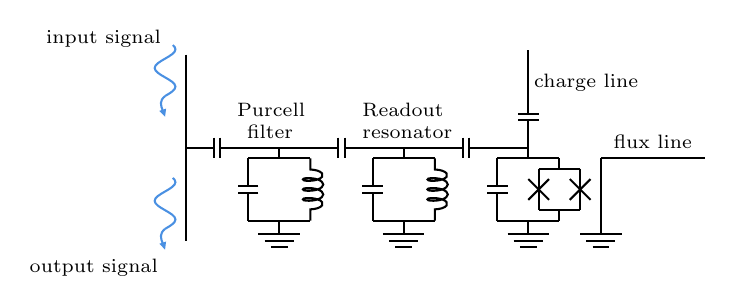
\begin{tikzpicture}[x=0.75pt,y=0.75pt,yscale=-1,xscale=1]
%uncomment if require: \path (0,300); %set diagram left start at 0, and has height of 300

%Shape: Capacitor [id:dp6229484510249941] 
\draw   (80,115) -- (93.5,115) (96.5,110) -- (96.5,120) (93.5,110) -- (93.5,120) (96.5,115) -- (110,115) ;
%Straight Lines [id:da5079772797363618] 
\draw    (140,120) -- (110,120) ;
%Shape: Inductor (Air Core) [id:dp10839806036975186] 
\draw   (140,120) -- (140,125.4) .. controls (142.63,125.48) and (144.87,126.23) .. (145.66,127.29) .. controls (146.44,128.35) and (145.61,129.5) .. (143.55,130.2) .. controls (141.95,130.74) and (139.88,130.95) .. (137.87,130.8) .. controls (137.08,130.8) and (136.45,130.53) .. (136.45,130.2) .. controls (136.45,129.87) and (137.08,129.6) .. (137.87,129.6) .. controls (139.88,129.45) and (141.95,129.66) .. (143.55,130.2) .. controls (145.26,130.82) and (146.23,131.69) .. (146.23,132.6) .. controls (146.23,133.51) and (145.26,134.38) .. (143.55,135) .. controls (141.95,135.54) and (139.88,135.75) .. (137.87,135.6) .. controls (137.08,135.6) and (136.45,135.33) .. (136.45,135) .. controls (136.45,134.67) and (137.08,134.4) .. (137.87,134.4) .. controls (139.88,134.25) and (141.95,134.46) .. (143.55,135) .. controls (145.26,135.62) and (146.23,136.49) .. (146.23,137.4) .. controls (146.23,138.31) and (145.26,139.18) .. (143.55,139.8) .. controls (141.95,140.34) and (139.88,140.55) .. (137.87,140.4) .. controls (137.08,140.4) and (136.45,140.13) .. (136.45,139.8) .. controls (136.45,139.47) and (137.08,139.2) .. (137.87,139.2) .. controls (139.88,139.05) and (141.95,139.26) .. (143.55,139.8) .. controls (145.61,140.5) and (146.44,141.65) .. (145.66,142.71) .. controls (144.87,143.77) and (142.63,144.52) .. (140,144.6) -- (140,150) ;
%Shape: Capacitor [id:dp06818692783071034] 
\draw   (110,120) -- (110,133.5) (115,136.5) -- (105,136.5) (115,133.5) -- (105,133.5) (110,136.5) -- (110,150) ;
%Straight Lines [id:da7350026547264685] 
\draw    (110,150) -- (140,150) ;
%Straight Lines [id:da23995913734624486] 
\draw    (80,70) -- (80,160) ;
%Straight Lines [id:da1612492392898659] 
\draw    (110,115) -- (140,115) ;
%Straight Lines [id:da5671640840709973] 
\draw    (125,115) -- (125,120) ;
%Shape: Capacitor [id:dp5438650003798182] 
\draw   (140,115) -- (153.5,115) (156.5,110) -- (156.5,120) (153.5,110) -- (153.5,120) (156.5,115) -- (170,115) ;
%Straight Lines [id:da49049414599623864] 
\draw    (200,120) -- (170,120) ;
%Shape: Inductor (Air Core) [id:dp010409349579149074] 
\draw   (200,120) -- (200,125.4) .. controls (202.63,125.48) and (204.87,126.23) .. (205.66,127.29) .. controls (206.44,128.35) and (205.61,129.5) .. (203.55,130.2) .. controls (201.95,130.74) and (199.88,130.95) .. (197.87,130.8) .. controls (197.08,130.8) and (196.45,130.53) .. (196.45,130.2) .. controls (196.45,129.87) and (197.08,129.6) .. (197.87,129.6) .. controls (199.88,129.45) and (201.95,129.66) .. (203.55,130.2) .. controls (205.26,130.82) and (206.23,131.69) .. (206.23,132.6) .. controls (206.23,133.51) and (205.26,134.38) .. (203.55,135) .. controls (201.95,135.54) and (199.88,135.75) .. (197.87,135.6) .. controls (197.08,135.6) and (196.45,135.33) .. (196.45,135) .. controls (196.45,134.67) and (197.08,134.4) .. (197.87,134.4) .. controls (199.88,134.25) and (201.95,134.46) .. (203.55,135) .. controls (205.26,135.62) and (206.23,136.49) .. (206.23,137.4) .. controls (206.23,138.31) and (205.26,139.18) .. (203.55,139.8) .. controls (201.95,140.34) and (199.88,140.55) .. (197.87,140.4) .. controls (197.08,140.4) and (196.45,140.13) .. (196.45,139.8) .. controls (196.45,139.47) and (197.08,139.2) .. (197.87,139.2) .. controls (199.88,139.05) and (201.95,139.26) .. (203.55,139.8) .. controls (205.61,140.5) and (206.44,141.65) .. (205.66,142.71) .. controls (204.87,143.77) and (202.63,144.52) .. (200,144.6) -- (200,150) ;
%Shape: Capacitor [id:dp38289405277156474] 
\draw   (170,120) -- (170,133.5) (175,136.5) -- (165,136.5) (175,133.5) -- (165,133.5) (170,136.5) -- (170,150) ;
%Straight Lines [id:da7342631646168638] 
\draw    (170,150) -- (200,150) ;
%Shape: Capacitor [id:dp4965705456609162] 
\draw   (200,115) -- (213.5,115) (216.5,110) -- (216.5,120) (213.5,110) -- (213.5,120) (216.5,115) -- (230,115) ;
%Straight Lines [id:da5477595668599946] 
\draw    (170,115) -- (200,115) ;
%Straight Lines [id:da7609436744451872] 
\draw    (185,115) -- (185,120) ;
%Straight Lines [id:da932132356010352] 
\draw    (260,120) -- (230,120) ;
%Shape: Capacitor [id:dp925083204210299] 
\draw   (230,120) -- (230,133.5) (235,136.5) -- (225,136.5) (235,133.5) -- (225,133.5) (230,136.5) -- (230,150) ;
%Straight Lines [id:da48756322841661204] 
\draw    (230,150) -- (260,150) ;
%Straight Lines [id:da9662762169593431] 
\draw    (245,115) -- (245,120) ;
%Straight Lines [id:da607486087129423] 
\draw    (250,125) -- (270,125) ;
%Straight Lines [id:da4269839144692542] 
\draw    (250,145) -- (270,145) ;
%Straight Lines [id:da6212379775483154] 
\draw    (270,125) -- (270,145) ;
%Straight Lines [id:da42941601462568646] 
\draw    (250,125) -- (250,145) ;
%Straight Lines [id:da9671029825944342] 
\draw    (260,120) -- (260,125) ;
%Straight Lines [id:da9712181495027408] 
\draw    (260,145) -- (260,150) ;
%Straight Lines [id:da3624697790998732] 
\draw    (265,130) -- (275,140) ;
%Straight Lines [id:da4335724022567018] 
\draw    (245,130) -- (255,140) ;
%Straight Lines [id:da530417781084312] 
\draw    (255,130) -- (245,140) ;
%Straight Lines [id:da9581131846208597] 
\draw    (275,130) -- (265,140) ;
%Straight Lines [id:da038301723534536425] 
\draw    (230,115) -- (245,115) ;
%Shape: Ground [id:dp6910953506421662] 
\draw   (115,156.67) -- (135,156.67) ;
\draw   (118,159.67) -- (132,159.67) ;
\draw   (121,162.67) -- (129,162.67) ;
\draw   (125,150) -- (125,156.67) ;
%Shape: Ground [id:dp4840755871676472] 
\draw   (175,156.67) -- (195,156.67) ;
\draw   (178,159.67) -- (192,159.67) ;
\draw   (181,162.67) -- (189,162.67) ;
\draw   (185,150) -- (185,156.67) ;
%Shape: Ground [id:dp7159028270026297] 
\draw   (235,156.67) -- (255,156.67) ;
\draw   (238,159.67) -- (252,159.67) ;
\draw   (241,162.67) -- (249,162.67) ;
\draw   (245,150) -- (245,156.67) ;
%Straight Lines [id:da07274023253816075] 
\draw    (280,120) -- (330,120) ;
%Straight Lines [id:da0646328748380458] 
\draw    (280,120) -- (280,150) ;
%Shape: Ground [id:dp10990759893272828] 
\draw   (270,156.67) -- (290,156.67) ;
\draw   (273,159.67) -- (287,159.67) ;
\draw   (276,162.67) -- (284,162.67) ;
\draw   (280,150) -- (280,156.67) ;
%Straight Lines [id:da8443452176258857] 
\draw    (245,68) -- (245,85) ;
%Shape: Capacitor [id:dp2673784375807502] 
\draw   (245,85) -- (245,98.5) (250,101.5) -- (240,101.5) (250,98.5) -- (240,98.5) (245,101.5) -- (245,115) ;
%Shape: Wave [id:dp46962992426174544] 
\draw  [color={rgb, 255:red, 74; green, 144; blue, 226 }  ,draw opacity=1 ] (70,90) .. controls (72.56,88.53) and (75,87.13) .. (75,85.5) .. controls (75,83.87) and (72.56,82.47) .. (70,81) .. controls (67.44,79.53) and (65,78.13) .. (65,76.5) .. controls (65,74.87) and (67.44,73.47) .. (70,72) .. controls (72.56,70.53) and (75,69.13) .. (75,67.5) .. controls (75,66.77) and (74.51,66.09) .. (73.75,65.43) ;
%Curve Lines [id:da8193635142444085] 
\draw [color={rgb, 255:red, 74; green, 144; blue, 226 }  ,draw opacity=1 ]   (70,90) .. controls (67.21,92.34) and (67.82,94.25) .. (68.96,97.21) ;
\draw [shift={(70,100)}, rotate = 251.57] [fill={rgb, 255:red, 74; green, 144; blue, 226 }  ,fill opacity=1 ][line width=0.08]  [draw opacity=0] (3.57,-1.72) -- (0,0) -- (3.57,1.72) -- cycle    ;
%Shape: Wave [id:dp5292058745377288] 
\draw  [color={rgb, 255:red, 74; green, 144; blue, 226 }  ,draw opacity=1 ] (70,154) .. controls (72.56,152.53) and (75,151.13) .. (75,149.5) .. controls (75,147.87) and (72.56,146.47) .. (70,145) .. controls (67.44,143.53) and (65,142.13) .. (65,140.5) .. controls (65,138.87) and (67.44,137.47) .. (70,136) .. controls (72.56,134.53) and (75,133.13) .. (75,131.5) .. controls (75,130.77) and (74.51,130.09) .. (73.75,129.43) ;
%Curve Lines [id:da04097203302843688] 
\draw [color={rgb, 255:red, 74; green, 144; blue, 226 }  ,draw opacity=1 ]   (70,154) .. controls (67.21,156.34) and (67.82,158.25) .. (68.96,161.21) ;
\draw [shift={(70,164)}, rotate = 251.57] [fill={rgb, 255:red, 74; green, 144; blue, 226 }  ,fill opacity=1 ][line width=0.08]  [draw opacity=0] (3.57,-1.72) -- (0,0) -- (3.57,1.72) -- cycle    ;

% Text Node
\draw (305,117) node [anchor=south] [inner sep=0.75pt]  [font=\scriptsize] [align=left] {{\scriptsize flux line}};
% Text Node
\draw (246.31,83.64) node [anchor=west] [inner sep=0.75pt]  [font=\scriptsize] [align=left] {{\scriptsize charge line}};
% Text Node
\draw (181,112) node [anchor=south] [inner sep=0.75pt]  [font=\scriptsize] [align=left] {\begin{minipage}[lt]{23.84pt}\setlength\topsep{0pt}
\begin{center}
{\scriptsize Readout}\\{\scriptsize resonator }
\end{center}

\end{minipage}};
% Text Node
\draw (138,112) node [anchor=south east] [inner sep=0.75pt]  [font=\scriptsize] [align=left] {\begin{minipage}[lt]{23.84pt}\setlength\topsep{0pt}
\begin{center}
{\scriptsize Purcell}\\{\scriptsize filter}
\end{center}

\end{minipage}};
% Text Node
\draw (69.47,67.86) node [anchor=south east] [inner sep=0.75pt]  [font=\scriptsize] [align=left] {{\scriptsize input signal}};
% Text Node
\draw (68,167) node [anchor=north east] [inner sep=0.75pt]  [font=\scriptsize] [align=left] {{\scriptsize output signal}};


\end{tikzpicture}


    \vspace{-1cm}
    \caption{Diagram representing a qubit together with flux line, charge line and readout mechanism}
    \label{fig:diagram_storage_qubit}
\end{figure}

%\begin{figure}
%    \centering
%    \begin{subfigure}{0.55\textwidth}
%        \centering
%        

\tikzset{every picture/.style={line width=0.75pt}} %set default line width to 0.75pt      

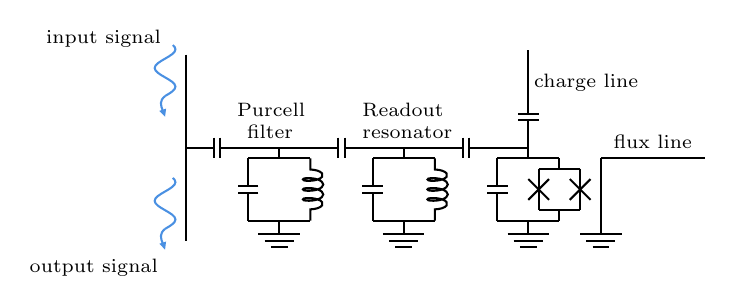
\begin{tikzpicture}[x=0.75pt,y=0.75pt,yscale=-1,xscale=1]
%uncomment if require: \path (0,300); %set diagram left start at 0, and has height of 300

%Shape: Capacitor [id:dp6229484510249941] 
\draw   (80,115) -- (93.5,115) (96.5,110) -- (96.5,120) (93.5,110) -- (93.5,120) (96.5,115) -- (110,115) ;
%Straight Lines [id:da5079772797363618] 
\draw    (140,120) -- (110,120) ;
%Shape: Inductor (Air Core) [id:dp10839806036975186] 
\draw   (140,120) -- (140,125.4) .. controls (142.63,125.48) and (144.87,126.23) .. (145.66,127.29) .. controls (146.44,128.35) and (145.61,129.5) .. (143.55,130.2) .. controls (141.95,130.74) and (139.88,130.95) .. (137.87,130.8) .. controls (137.08,130.8) and (136.45,130.53) .. (136.45,130.2) .. controls (136.45,129.87) and (137.08,129.6) .. (137.87,129.6) .. controls (139.88,129.45) and (141.95,129.66) .. (143.55,130.2) .. controls (145.26,130.82) and (146.23,131.69) .. (146.23,132.6) .. controls (146.23,133.51) and (145.26,134.38) .. (143.55,135) .. controls (141.95,135.54) and (139.88,135.75) .. (137.87,135.6) .. controls (137.08,135.6) and (136.45,135.33) .. (136.45,135) .. controls (136.45,134.67) and (137.08,134.4) .. (137.87,134.4) .. controls (139.88,134.25) and (141.95,134.46) .. (143.55,135) .. controls (145.26,135.62) and (146.23,136.49) .. (146.23,137.4) .. controls (146.23,138.31) and (145.26,139.18) .. (143.55,139.8) .. controls (141.95,140.34) and (139.88,140.55) .. (137.87,140.4) .. controls (137.08,140.4) and (136.45,140.13) .. (136.45,139.8) .. controls (136.45,139.47) and (137.08,139.2) .. (137.87,139.2) .. controls (139.88,139.05) and (141.95,139.26) .. (143.55,139.8) .. controls (145.61,140.5) and (146.44,141.65) .. (145.66,142.71) .. controls (144.87,143.77) and (142.63,144.52) .. (140,144.6) -- (140,150) ;
%Shape: Capacitor [id:dp06818692783071034] 
\draw   (110,120) -- (110,133.5) (115,136.5) -- (105,136.5) (115,133.5) -- (105,133.5) (110,136.5) -- (110,150) ;
%Straight Lines [id:da7350026547264685] 
\draw    (110,150) -- (140,150) ;
%Straight Lines [id:da23995913734624486] 
\draw    (80,70) -- (80,160) ;
%Straight Lines [id:da1612492392898659] 
\draw    (110,115) -- (140,115) ;
%Straight Lines [id:da5671640840709973] 
\draw    (125,115) -- (125,120) ;
%Shape: Capacitor [id:dp5438650003798182] 
\draw   (140,115) -- (153.5,115) (156.5,110) -- (156.5,120) (153.5,110) -- (153.5,120) (156.5,115) -- (170,115) ;
%Straight Lines [id:da49049414599623864] 
\draw    (200,120) -- (170,120) ;
%Shape: Inductor (Air Core) [id:dp010409349579149074] 
\draw   (200,120) -- (200,125.4) .. controls (202.63,125.48) and (204.87,126.23) .. (205.66,127.29) .. controls (206.44,128.35) and (205.61,129.5) .. (203.55,130.2) .. controls (201.95,130.74) and (199.88,130.95) .. (197.87,130.8) .. controls (197.08,130.8) and (196.45,130.53) .. (196.45,130.2) .. controls (196.45,129.87) and (197.08,129.6) .. (197.87,129.6) .. controls (199.88,129.45) and (201.95,129.66) .. (203.55,130.2) .. controls (205.26,130.82) and (206.23,131.69) .. (206.23,132.6) .. controls (206.23,133.51) and (205.26,134.38) .. (203.55,135) .. controls (201.95,135.54) and (199.88,135.75) .. (197.87,135.6) .. controls (197.08,135.6) and (196.45,135.33) .. (196.45,135) .. controls (196.45,134.67) and (197.08,134.4) .. (197.87,134.4) .. controls (199.88,134.25) and (201.95,134.46) .. (203.55,135) .. controls (205.26,135.62) and (206.23,136.49) .. (206.23,137.4) .. controls (206.23,138.31) and (205.26,139.18) .. (203.55,139.8) .. controls (201.95,140.34) and (199.88,140.55) .. (197.87,140.4) .. controls (197.08,140.4) and (196.45,140.13) .. (196.45,139.8) .. controls (196.45,139.47) and (197.08,139.2) .. (197.87,139.2) .. controls (199.88,139.05) and (201.95,139.26) .. (203.55,139.8) .. controls (205.61,140.5) and (206.44,141.65) .. (205.66,142.71) .. controls (204.87,143.77) and (202.63,144.52) .. (200,144.6) -- (200,150) ;
%Shape: Capacitor [id:dp38289405277156474] 
\draw   (170,120) -- (170,133.5) (175,136.5) -- (165,136.5) (175,133.5) -- (165,133.5) (170,136.5) -- (170,150) ;
%Straight Lines [id:da7342631646168638] 
\draw    (170,150) -- (200,150) ;
%Shape: Capacitor [id:dp4965705456609162] 
\draw   (200,115) -- (213.5,115) (216.5,110) -- (216.5,120) (213.5,110) -- (213.5,120) (216.5,115) -- (230,115) ;
%Straight Lines [id:da5477595668599946] 
\draw    (170,115) -- (200,115) ;
%Straight Lines [id:da7609436744451872] 
\draw    (185,115) -- (185,120) ;
%Straight Lines [id:da932132356010352] 
\draw    (260,120) -- (230,120) ;
%Shape: Capacitor [id:dp925083204210299] 
\draw   (230,120) -- (230,133.5) (235,136.5) -- (225,136.5) (235,133.5) -- (225,133.5) (230,136.5) -- (230,150) ;
%Straight Lines [id:da48756322841661204] 
\draw    (230,150) -- (260,150) ;
%Straight Lines [id:da9662762169593431] 
\draw    (245,115) -- (245,120) ;
%Straight Lines [id:da607486087129423] 
\draw    (250,125) -- (270,125) ;
%Straight Lines [id:da4269839144692542] 
\draw    (250,145) -- (270,145) ;
%Straight Lines [id:da6212379775483154] 
\draw    (270,125) -- (270,145) ;
%Straight Lines [id:da42941601462568646] 
\draw    (250,125) -- (250,145) ;
%Straight Lines [id:da9671029825944342] 
\draw    (260,120) -- (260,125) ;
%Straight Lines [id:da9712181495027408] 
\draw    (260,145) -- (260,150) ;
%Straight Lines [id:da3624697790998732] 
\draw    (265,130) -- (275,140) ;
%Straight Lines [id:da4335724022567018] 
\draw    (245,130) -- (255,140) ;
%Straight Lines [id:da530417781084312] 
\draw    (255,130) -- (245,140) ;
%Straight Lines [id:da9581131846208597] 
\draw    (275,130) -- (265,140) ;
%Straight Lines [id:da038301723534536425] 
\draw    (230,115) -- (245,115) ;
%Shape: Ground [id:dp6910953506421662] 
\draw   (115,156.67) -- (135,156.67) ;
\draw   (118,159.67) -- (132,159.67) ;
\draw   (121,162.67) -- (129,162.67) ;
\draw   (125,150) -- (125,156.67) ;
%Shape: Ground [id:dp4840755871676472] 
\draw   (175,156.67) -- (195,156.67) ;
\draw   (178,159.67) -- (192,159.67) ;
\draw   (181,162.67) -- (189,162.67) ;
\draw   (185,150) -- (185,156.67) ;
%Shape: Ground [id:dp7159028270026297] 
\draw   (235,156.67) -- (255,156.67) ;
\draw   (238,159.67) -- (252,159.67) ;
\draw   (241,162.67) -- (249,162.67) ;
\draw   (245,150) -- (245,156.67) ;
%Straight Lines [id:da07274023253816075] 
\draw    (280,120) -- (330,120) ;
%Straight Lines [id:da0646328748380458] 
\draw    (280,120) -- (280,150) ;
%Shape: Ground [id:dp10990759893272828] 
\draw   (270,156.67) -- (290,156.67) ;
\draw   (273,159.67) -- (287,159.67) ;
\draw   (276,162.67) -- (284,162.67) ;
\draw   (280,150) -- (280,156.67) ;
%Straight Lines [id:da8443452176258857] 
\draw    (245,68) -- (245,85) ;
%Shape: Capacitor [id:dp2673784375807502] 
\draw   (245,85) -- (245,98.5) (250,101.5) -- (240,101.5) (250,98.5) -- (240,98.5) (245,101.5) -- (245,115) ;
%Shape: Wave [id:dp46962992426174544] 
\draw  [color={rgb, 255:red, 74; green, 144; blue, 226 }  ,draw opacity=1 ] (70,90) .. controls (72.56,88.53) and (75,87.13) .. (75,85.5) .. controls (75,83.87) and (72.56,82.47) .. (70,81) .. controls (67.44,79.53) and (65,78.13) .. (65,76.5) .. controls (65,74.87) and (67.44,73.47) .. (70,72) .. controls (72.56,70.53) and (75,69.13) .. (75,67.5) .. controls (75,66.77) and (74.51,66.09) .. (73.75,65.43) ;
%Curve Lines [id:da8193635142444085] 
\draw [color={rgb, 255:red, 74; green, 144; blue, 226 }  ,draw opacity=1 ]   (70,90) .. controls (67.21,92.34) and (67.82,94.25) .. (68.96,97.21) ;
\draw [shift={(70,100)}, rotate = 251.57] [fill={rgb, 255:red, 74; green, 144; blue, 226 }  ,fill opacity=1 ][line width=0.08]  [draw opacity=0] (3.57,-1.72) -- (0,0) -- (3.57,1.72) -- cycle    ;
%Shape: Wave [id:dp5292058745377288] 
\draw  [color={rgb, 255:red, 74; green, 144; blue, 226 }  ,draw opacity=1 ] (70,154) .. controls (72.56,152.53) and (75,151.13) .. (75,149.5) .. controls (75,147.87) and (72.56,146.47) .. (70,145) .. controls (67.44,143.53) and (65,142.13) .. (65,140.5) .. controls (65,138.87) and (67.44,137.47) .. (70,136) .. controls (72.56,134.53) and (75,133.13) .. (75,131.5) .. controls (75,130.77) and (74.51,130.09) .. (73.75,129.43) ;
%Curve Lines [id:da04097203302843688] 
\draw [color={rgb, 255:red, 74; green, 144; blue, 226 }  ,draw opacity=1 ]   (70,154) .. controls (67.21,156.34) and (67.82,158.25) .. (68.96,161.21) ;
\draw [shift={(70,164)}, rotate = 251.57] [fill={rgb, 255:red, 74; green, 144; blue, 226 }  ,fill opacity=1 ][line width=0.08]  [draw opacity=0] (3.57,-1.72) -- (0,0) -- (3.57,1.72) -- cycle    ;

% Text Node
\draw (305,117) node [anchor=south] [inner sep=0.75pt]  [font=\scriptsize] [align=left] {{\scriptsize flux line}};
% Text Node
\draw (246.31,83.64) node [anchor=west] [inner sep=0.75pt]  [font=\scriptsize] [align=left] {{\scriptsize charge line}};
% Text Node
\draw (181,112) node [anchor=south] [inner sep=0.75pt]  [font=\scriptsize] [align=left] {\begin{minipage}[lt]{23.84pt}\setlength\topsep{0pt}
\begin{center}
{\scriptsize Readout}\\{\scriptsize resonator }
\end{center}

\end{minipage}};
% Text Node
\draw (138,112) node [anchor=south east] [inner sep=0.75pt]  [font=\scriptsize] [align=left] {\begin{minipage}[lt]{23.84pt}\setlength\topsep{0pt}
\begin{center}
{\scriptsize Purcell}\\{\scriptsize filter}
\end{center}

\end{minipage}};
% Text Node
\draw (69.47,67.86) node [anchor=south east] [inner sep=0.75pt]  [font=\scriptsize] [align=left] {{\scriptsize input signal}};
% Text Node
\draw (68,167) node [anchor=north east] [inner sep=0.75pt]  [font=\scriptsize] [align=left] {{\scriptsize output signal}};


\end{tikzpicture}


%        \vspace{-1cm}
%        \caption{Diagram representing a qubit together with flux line, charge line and readout mechanism}
%        \label{fig:diagram_storage_qubit}
%    \end{subfigure}
%    \hspace{0.3cm}
%    \begin{subfigure}{0.35\textwidth}
%        \centering
%        \includegraphics[width=\textwidth]{Images/Chap1/Readout_pic.png} 
%        \caption{Micrograph}
%        \label{fig:diagram_storage_qubit_real}
%    \end{subfigure}
%    \caption{A qubit together with flux line, charge line and readout mechanism}
%    \label{fig:diagram_storage_qubit_tot}
%\end{figure}

\subsection{Charge line}

The \emph{charge line} serves to execute single-qubit gates on the transmon qubit.
It is capacitively linked to the central island of the qubit.
A coherent drive of time-dependent amplitude $\varepsilon(t)$, frequency $\omega_d$ and phase $\phi_d$ is modeled by the Hamiltonian \cite{LC_resonator}
\begin{equation}
    \hat{H} = \frac{\hbar \delta}{2} \hat{\sigma}_z + 
    \hbar \varepsilon(t) \left( \cos(\phi_d) \hat{\sigma}_x + \sin(\phi_d) \hat{\sigma}_y \right) ,
\end{equation}
where the Hamiltonian is expressed within a frame rotating at $\omega_d$, and $\delta$ represents the detuning between the qubit and the drive. 
This illustrates how the phase $\phi_d$ of the drive enables the selection of rotations around either the $x$ or $y$ axis. 
For example, when $\delta = 0$, setting $\phi_d = 0$ executes a rotation around the $x$ axis, while $\phi = \pi/2$ corresponds to a rotation around the $y$ axis. 
Given that any rotation on the Bloch sphere can be decomposed into rotations around two axes, we can implement any single-qubit gate by sequencing the appropriate gates with the corresponding phases.

\subsection{Readout resonator}

The readout mechanism comprises two primary components: the \emph{readout resonator} and the \emph{Purcell filter}. 
Its objective is to measure the state of the qubit in a non-destructive manner \cite{singleshot_readout}.

The starting point is the famous Jaynes-Cummings Hamiltonian \cite{haroche2006exploring}
\begin{equation}
    \hat{H} = \hbar \omega_r \hat{a}^\dagger \hat{a} + \frac{1}{2} \hbar \omega_{ge} \hat{\sigma}_z + \hbar g (\hat{a}^\dagger \hat{\sigma}^- + \hat{a} \hat{\sigma}^+) ,
\end{equation}
which models the interaction between a two-level system with transition frequency $\omega_{ge}$ and an electromagnetic field mode at frequency $\omega_r$.
In the dispersive regime ($|\omega_r - \omega_{ge} \gg g|$), the Hamiltonian reduces to \cite{transmon_regime}
\begin{align}
    \hat{H} &= \hbar \omega_r \hat{a}^\dagger \hat{a} + \frac{1}{2} \hbar \omega_{ge} \hat{\sigma}_z + \hbar \chi \hat{\sigma}_z \hat{a}^\dagger \hat{a} \\
    &= \hbar (\omega_r + \chi \hat{\sigma}_z ) \hat{a}^\dagger \hat{a} +
    \frac{1}{2} \hbar \omega_{ge} \hat{\sigma}_z 
\end{align}
where $\chi$ is the qubit-state dependent cavity-shift.

Thus, the resonator's frequency becomes qubit-state's dependent.
If, for instance, the qubit is in the $\ket{g}$ state, then the resonator's frequency will become $\omega_r - \chi$.
On the other hand, if the qubit is in the $\ket{e}$ state, then the resonator's frequency will be $\omega_r + \chi$.
The frequency of the resonator can be determined by assessing the transmission of an input signal through the feedline (see \cref{fig:diagram_storage_qubit}).
This transmission decreases when the signal is on resonance with the resonator's frequency.

In case where the qubit is in a mixed state like
\begin{equation}
    c_g \ket{g} + c_e \ket{e} ,
\end{equation}
then driving the resonator would results in an entangled state between the coherent signal and the qubit
\begin{equation}
    c_g \ket{g, \alpha_g} + c_e \ket{e, \alpha_e} .
\end{equation}
Thus, measuring either $\alpha_g$ or $\alpha_e$ will collapse the state of the qubit onto $\ket{g}$ or $\ket{e}$, respectively.
The principle underlying quantum non-demolition (QND) measurement is predicated on the stability of the state post-measurement.
This implies that subsequent QND measurements would yield identical results, as the state remains unchanged.

To prevent excessive coupling between the qubit and its environment via the readout resonator, a Purcell filter is interposed between them.
This configuration helps extend the qubit lifetimes by mitigating spontaneous emission resulting from the Purcell effect \cite{Purcell_effect}.

\subsection{Tunable couplers}

\begin{figure}
    \centering
    \begin{subfigure}{0.65\textwidth}
        \centering
        

\tikzset{every picture/.style={line width=0.75pt}} %set default line width to 0.75pt        

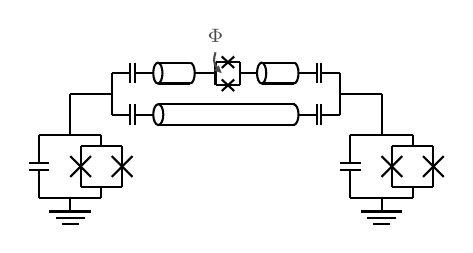
\begin{tikzpicture}[x=0.75pt,y=0.75pt,yscale=-1,xscale=1]
%uncomment if require: \path (0,300); %set diagram left start at 0, and has height of 300

%Straight Lines [id:da07218492708859259] 
\draw    (165,140) -- (135,140) ;
%Shape: Capacitor [id:dp26518043172092054] 
\draw   (135,140) -- (135,153.5) (140,156.5) -- (130,156.5) (140,153.5) -- (130,153.5) (135,156.5) -- (135,170) ;
%Straight Lines [id:da13302415031214743] 
\draw    (135,170) -- (165,170) ;
%Straight Lines [id:da17130629114618245] 
\draw    (155,145) -- (175,145) ;
%Straight Lines [id:da29260280538604033] 
\draw    (155,165) -- (175,165) ;
%Straight Lines [id:da49230231307780326] 
\draw    (175,145) -- (175,165) ;
%Straight Lines [id:da3653947605727903] 
\draw    (155,145) -- (155,165) ;
%Straight Lines [id:da44803766219329755] 
\draw    (165,140) -- (165,145) ;
%Straight Lines [id:da9101556277746032] 
\draw    (165,165) -- (165,170) ;
%Straight Lines [id:da006475878830819681] 
\draw    (170,150) -- (180,160) ;
%Straight Lines [id:da33120831736226397] 
\draw    (150,150) -- (160,160) ;
%Straight Lines [id:da11004761294731558] 
\draw    (160,150) -- (150,160) ;
%Straight Lines [id:da9445264009597942] 
\draw    (180,150) -- (170,160) ;
%Shape: Ground [id:dp22167919288849824] 
\draw   (140, 176.67) -- (160, 176.67) ;
\draw   (143, 179.67) -- (157, 179.67) ;
\draw   (146, 182.67) -- (154, 182.67) ;
\draw   (150, 170) -- (150, 176.67) ;
%Straight Lines [id:da42940827257352] 
\draw    (315,140) -- (285,140) ;
%Shape: Capacitor [id:dp49877304955829627] 
\draw   (285,140) -- (285,153.5) (290,156.5) -- (280,156.5) (290,153.5) -- (280,153.5) (285,156.5) -- (285,170) ;
%Straight Lines [id:da7324100328789034] 
\draw    (285,170) -- (315,170) ;
%Straight Lines [id:da208048098521316] 
\draw    (305,145) -- (325,145) ;
%Straight Lines [id:da8572518030578566] 
\draw    (305,165) -- (325,165) ;
%Straight Lines [id:da5742858039200953] 
\draw    (325,145) -- (325,165) ;
%Straight Lines [id:da3966431831849069] 
\draw    (305,145) -- (305,165) ;
%Straight Lines [id:da19183525795672862] 
\draw    (315,140) -- (315,145) ;
%Straight Lines [id:da004743615923411104] 
\draw    (315,165) -- (315,170) ;
%Straight Lines [id:da17738152912719607] 
\draw    (320,150) -- (330,160) ;
%Straight Lines [id:da8678835567326026] 
\draw    (300,150) -- (310,160) ;
%Straight Lines [id:da28374358820735224] 
\draw    (310,150) -- (300,160) ;
%Straight Lines [id:da24817307713778236] 
\draw    (330,150) -- (320,160) ;
%Shape: Ground [id:dp861700376356459] 
\draw   (290, 176.67) -- (310, 176.67) ;
\draw   (293, 179.67) -- (307, 179.67) ;
\draw   (296, 182.67) -- (304, 182.67) ;
\draw   (300, 170) -- (300, 176.67) ;
%Straight Lines [id:da6625685419222695] 
\draw    (150,140) -- (150,120) ;
%Straight Lines [id:da2635718281625268] 
\draw    (300,140) -- (300,120) ;
%Straight Lines [id:da3980890926472094] 
\draw    (170,120) -- (150,120) ;
%Straight Lines [id:da6516978234304753] 
\draw    (170,120) -- (170,110) ;
%Straight Lines [id:da8682527218489697] 
\draw    (170,130) -- (170,120) ;
%Shape: Capacitor [id:dp26464751353501326] 
\draw   (170,110) -- (179,110) (181,105) -- (181,115) (179,105) -- (179,115) (181,110) -- (190,110) ;
%Shape: Capacitor [id:dp9673816527519772] 
\draw   (170,130) -- (179,130) (181,125) -- (181,135) (179,125) -- (179,135) (181,130) -- (190,130) ;
%Shape: Ellipse [id:dp26511497109868176] 
\draw   (190,110) .. controls (190,107.24) and (191,105) .. (192.22,105) .. controls (193.45,105) and (194.45,107.24) .. (194.45,110) .. controls (194.45,112.76) and (193.45,115) .. (192.22,115) .. controls (191,115) and (190,112.76) .. (190,110) -- cycle ;
%Straight Lines [id:da14470289747688758] 
\draw    (192.22,105) -- (207.79,105) ;
%Straight Lines [id:da773223714503521] 
\draw    (192.22,115) -- (207.79,115) ;
%Shape: Arc [id:dp18440292021788673] 
\draw  [draw opacity=0] (207.79,105) .. controls (209.01,105.02) and (210,107.25) .. (210,110) .. controls (210,112.75) and (209.01,114.98) .. (207.79,115) -- (207.78,110) -- cycle ; \draw   (207.79,105) .. controls (209.01,105.02) and (210,107.25) .. (210,110) .. controls (210,112.75) and (209.01,114.98) .. (207.79,115) ;  

%Shape: Ellipse [id:dp6247106434937635] 
\draw   (190,130) .. controls (190,127.24) and (191.09,125) .. (192.43,125) .. controls (193.77,125) and (194.86,127.24) .. (194.86,130) .. controls (194.86,132.76) and (193.77,135) .. (192.43,135) .. controls (191.09,135) and (190,132.76) .. (190,130) -- cycle ;
%Straight Lines [id:da5902234364980534] 
\draw    (192.43,125) -- (258.06,125) ;
%Straight Lines [id:da6759349880739789] 
\draw    (192.43,135) -- (258.06,135) ;
%Shape: Arc [id:dp6456040885907672] 
\draw  [draw opacity=0] (257.59,125) .. controls (258.92,125.02) and (260,127.25) .. (260,130) .. controls (260,132.75) and (258.92,134.98) .. (257.59,135) -- (257.57,130) -- cycle ; \draw   (257.59,125) .. controls (258.92,125.02) and (260,127.25) .. (260,130) .. controls (260,132.75) and (258.92,134.98) .. (257.59,135) ;  

%Shape: Ellipse [id:dp7275157055864581] 
\draw   (240,110) .. controls (240,107.24) and (241,105) .. (242.22,105) .. controls (243.45,105) and (244.45,107.24) .. (244.45,110) .. controls (244.45,112.76) and (243.45,115) .. (242.22,115) .. controls (241,115) and (240,112.76) .. (240,110) -- cycle ;
%Straight Lines [id:da6315731480773339] 
\draw    (242.22,105) -- (257.79,105) ;
%Straight Lines [id:da6406460700415237] 
\draw    (242.22,115) -- (257.79,115) ;
%Shape: Arc [id:dp38475017613626794] 
\draw  [draw opacity=0] (257.79,105) .. controls (259.01,105.02) and (260,107.25) .. (260,110) .. controls (260,112.75) and (259.01,114.98) .. (257.79,115) -- (257.78,110) -- cycle ; \draw   (257.79,105) .. controls (259.01,105.02) and (260,107.25) .. (260,110) .. controls (260,112.75) and (259.01,114.98) .. (257.79,115) ;  

%Straight Lines [id:da060781913550373545] 
\draw    (210,110) -- (220,110) ;
%Straight Lines [id:da15398066157627577] 
\draw    (232,104.77) -- (232,115.85) ;
%Straight Lines [id:da14222494293706922] 
\draw    (220,104.77) -- (220,115.85) ;
%Straight Lines [id:da6561755710145185] 
\draw    (232,115.85) -- (220,115.85) ;
%Straight Lines [id:da742586164519965] 
\draw    (232,104.77) -- (220,104.77) ;
%Straight Lines [id:da21146645385961227] 
\draw    (229,113.08) -- (223,118.63) ;
%Straight Lines [id:da3871753118676642] 
\draw    (229,102) -- (223,107.54) ;
%Straight Lines [id:da5637422527324993] 
\draw    (229,107.54) -- (223,102) ;
%Straight Lines [id:da9093097576487559] 
\draw    (229,118.63) -- (223,113.08) ;

%Straight Lines [id:da4289728577327423] 
\draw    (232,110) -- (240,110) ;
%Shape: Capacitor [id:dp8421236410162245] 
\draw   (260,110) -- (269,110) (271,105) -- (271,115) (269,105) -- (269,115) (271,110) -- (280,110) ;
%Straight Lines [id:da787480793091047] 
\draw    (280,120) -- (280,110) ;
%Straight Lines [id:da5372127440829679] 
\draw    (280,130) -- (280,120) ;
%Shape: Capacitor [id:dp09893187150822791] 
\draw   (260,130) -- (269,130) (271,125) -- (271,135) (269,125) -- (269,135) (271,130) -- (280,130) ;
%Straight Lines [id:da43455598058651357] 
\draw    (300,120) -- (280,120) ;
%Curve Lines [id:da7527622826730622] 
\draw [color={rgb, 255:red, 74; green, 74; blue, 74 }  ,draw opacity=1 ]   (220,100) .. controls (219.34,102.74) and (218.4,104.58) .. (220.96,107.82) ;
\draw [shift={(223,110)}, rotate = 223.23] [fill={rgb, 255:red, 74; green, 74; blue, 74 }  ,fill opacity=1 ][line width=0.08]  [draw opacity=0] (3.57,-1.72) -- (0,0) -- (3.57,1.72) -- cycle    ;

% Text Node
\draw (220,97) node [anchor=south] [inner sep=0.75pt]  [font=\scriptsize,color={rgb, 255:red, 74; green, 74; blue, 74 }  ,opacity=1 ] [align=left] {$\displaystyle \Phi $};


\end{tikzpicture}
        \vspace{-1cm}
        \caption{Diagram}
        \label{fig:tun_coupl}
    \end{subfigure}
    \hspace{0.3cm}
    \begin{subfigure}{0.25\textwidth}
        \centering
        \includegraphics[width=\textwidth]{Images/Chap1/tun_couplers.png} 
        \caption{Micrograph}
        \label{fig:tun_coupl_real}
    \end{subfigure}
    \caption{Two qubits connected by tunable couplers}
    \label{fig:tun_coupl_tot}
\end{figure}

We employ \emph{tunable couplers} \cite{tun_coupler} to control interactions between pairs of qubits.
They allow us to mediate interaction between the qubits and perform two-qubits gates.
They are composed of two coplanar waveguides (see \cref{fig:tun_coupl}).
One of them is a normal waveguide, and thus has a fixed coupling term $J_\text{fixed}$.
The other has a SQUID loop and is flux tunable.
Its coupling term $J_\text{tunable}(\phi)$ can be tuned with the magnetic flux generated by a flux line and going into a SQUID loop placed on the waveguide

The SQUID loop connected to the coupler allows us to control the interaction between the two qubits. 
To minimise the interaction between the two qubits and the ZZ crosstalk, the DC flux driving the SQUID loop has to be calibrated to the operation point.

To implement a two-qubit gate, a sinusoidal pulse is sent on top of the DC flux to the SQUID loop. If the modulation frequency of this pulse matches a transition of the two-qubit system, it will perform a two-qubit gate.
In this way we are able to turn on interactions between specific levels of the qubits (see \cref{chap:2_qubit_gates}).
\section{Tunable Couplers}
\label{sec:tunable_couplers}

Qubits in our device are coupled through tunable couplers.
They allow us to mediate interaction between the qubits and perform two-qubits gates.
They are composed of two planar waveguide, one of them with a fixed coupling term $J_{\text{fixed}}$.
The other is instead flux tunable, meaning that its coupling term $J_{\text{tunable}}(\Phi)$ can be tuned with the magnetic flux generated by a flux line and going into a SQUID loop placed on the waveguide as depicted in \cref{fig:tun_coupl}.

\begin{figure}
    \centering
    

\tikzset{every picture/.style={line width=0.75pt}} %set default line width to 0.75pt        

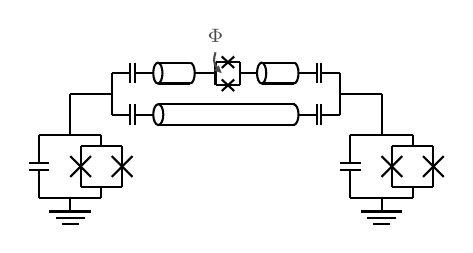
\begin{tikzpicture}[x=0.75pt,y=0.75pt,yscale=-1,xscale=1]
%uncomment if require: \path (0,300); %set diagram left start at 0, and has height of 300

%Straight Lines [id:da07218492708859259] 
\draw    (165,140) -- (135,140) ;
%Shape: Capacitor [id:dp26518043172092054] 
\draw   (135,140) -- (135,153.5) (140,156.5) -- (130,156.5) (140,153.5) -- (130,153.5) (135,156.5) -- (135,170) ;
%Straight Lines [id:da13302415031214743] 
\draw    (135,170) -- (165,170) ;
%Straight Lines [id:da17130629114618245] 
\draw    (155,145) -- (175,145) ;
%Straight Lines [id:da29260280538604033] 
\draw    (155,165) -- (175,165) ;
%Straight Lines [id:da49230231307780326] 
\draw    (175,145) -- (175,165) ;
%Straight Lines [id:da3653947605727903] 
\draw    (155,145) -- (155,165) ;
%Straight Lines [id:da44803766219329755] 
\draw    (165,140) -- (165,145) ;
%Straight Lines [id:da9101556277746032] 
\draw    (165,165) -- (165,170) ;
%Straight Lines [id:da006475878830819681] 
\draw    (170,150) -- (180,160) ;
%Straight Lines [id:da33120831736226397] 
\draw    (150,150) -- (160,160) ;
%Straight Lines [id:da11004761294731558] 
\draw    (160,150) -- (150,160) ;
%Straight Lines [id:da9445264009597942] 
\draw    (180,150) -- (170,160) ;
%Shape: Ground [id:dp22167919288849824] 
\draw   (140, 176.67) -- (160, 176.67) ;
\draw   (143, 179.67) -- (157, 179.67) ;
\draw   (146, 182.67) -- (154, 182.67) ;
\draw   (150, 170) -- (150, 176.67) ;
%Straight Lines [id:da42940827257352] 
\draw    (315,140) -- (285,140) ;
%Shape: Capacitor [id:dp49877304955829627] 
\draw   (285,140) -- (285,153.5) (290,156.5) -- (280,156.5) (290,153.5) -- (280,153.5) (285,156.5) -- (285,170) ;
%Straight Lines [id:da7324100328789034] 
\draw    (285,170) -- (315,170) ;
%Straight Lines [id:da208048098521316] 
\draw    (305,145) -- (325,145) ;
%Straight Lines [id:da8572518030578566] 
\draw    (305,165) -- (325,165) ;
%Straight Lines [id:da5742858039200953] 
\draw    (325,145) -- (325,165) ;
%Straight Lines [id:da3966431831849069] 
\draw    (305,145) -- (305,165) ;
%Straight Lines [id:da19183525795672862] 
\draw    (315,140) -- (315,145) ;
%Straight Lines [id:da004743615923411104] 
\draw    (315,165) -- (315,170) ;
%Straight Lines [id:da17738152912719607] 
\draw    (320,150) -- (330,160) ;
%Straight Lines [id:da8678835567326026] 
\draw    (300,150) -- (310,160) ;
%Straight Lines [id:da28374358820735224] 
\draw    (310,150) -- (300,160) ;
%Straight Lines [id:da24817307713778236] 
\draw    (330,150) -- (320,160) ;
%Shape: Ground [id:dp861700376356459] 
\draw   (290, 176.67) -- (310, 176.67) ;
\draw   (293, 179.67) -- (307, 179.67) ;
\draw   (296, 182.67) -- (304, 182.67) ;
\draw   (300, 170) -- (300, 176.67) ;
%Straight Lines [id:da6625685419222695] 
\draw    (150,140) -- (150,120) ;
%Straight Lines [id:da2635718281625268] 
\draw    (300,140) -- (300,120) ;
%Straight Lines [id:da3980890926472094] 
\draw    (170,120) -- (150,120) ;
%Straight Lines [id:da6516978234304753] 
\draw    (170,120) -- (170,110) ;
%Straight Lines [id:da8682527218489697] 
\draw    (170,130) -- (170,120) ;
%Shape: Capacitor [id:dp26464751353501326] 
\draw   (170,110) -- (179,110) (181,105) -- (181,115) (179,105) -- (179,115) (181,110) -- (190,110) ;
%Shape: Capacitor [id:dp9673816527519772] 
\draw   (170,130) -- (179,130) (181,125) -- (181,135) (179,125) -- (179,135) (181,130) -- (190,130) ;
%Shape: Ellipse [id:dp26511497109868176] 
\draw   (190,110) .. controls (190,107.24) and (191,105) .. (192.22,105) .. controls (193.45,105) and (194.45,107.24) .. (194.45,110) .. controls (194.45,112.76) and (193.45,115) .. (192.22,115) .. controls (191,115) and (190,112.76) .. (190,110) -- cycle ;
%Straight Lines [id:da14470289747688758] 
\draw    (192.22,105) -- (207.79,105) ;
%Straight Lines [id:da773223714503521] 
\draw    (192.22,115) -- (207.79,115) ;
%Shape: Arc [id:dp18440292021788673] 
\draw  [draw opacity=0] (207.79,105) .. controls (209.01,105.02) and (210,107.25) .. (210,110) .. controls (210,112.75) and (209.01,114.98) .. (207.79,115) -- (207.78,110) -- cycle ; \draw   (207.79,105) .. controls (209.01,105.02) and (210,107.25) .. (210,110) .. controls (210,112.75) and (209.01,114.98) .. (207.79,115) ;  

%Shape: Ellipse [id:dp6247106434937635] 
\draw   (190,130) .. controls (190,127.24) and (191.09,125) .. (192.43,125) .. controls (193.77,125) and (194.86,127.24) .. (194.86,130) .. controls (194.86,132.76) and (193.77,135) .. (192.43,135) .. controls (191.09,135) and (190,132.76) .. (190,130) -- cycle ;
%Straight Lines [id:da5902234364980534] 
\draw    (192.43,125) -- (258.06,125) ;
%Straight Lines [id:da6759349880739789] 
\draw    (192.43,135) -- (258.06,135) ;
%Shape: Arc [id:dp6456040885907672] 
\draw  [draw opacity=0] (257.59,125) .. controls (258.92,125.02) and (260,127.25) .. (260,130) .. controls (260,132.75) and (258.92,134.98) .. (257.59,135) -- (257.57,130) -- cycle ; \draw   (257.59,125) .. controls (258.92,125.02) and (260,127.25) .. (260,130) .. controls (260,132.75) and (258.92,134.98) .. (257.59,135) ;  

%Shape: Ellipse [id:dp7275157055864581] 
\draw   (240,110) .. controls (240,107.24) and (241,105) .. (242.22,105) .. controls (243.45,105) and (244.45,107.24) .. (244.45,110) .. controls (244.45,112.76) and (243.45,115) .. (242.22,115) .. controls (241,115) and (240,112.76) .. (240,110) -- cycle ;
%Straight Lines [id:da6315731480773339] 
\draw    (242.22,105) -- (257.79,105) ;
%Straight Lines [id:da6406460700415237] 
\draw    (242.22,115) -- (257.79,115) ;
%Shape: Arc [id:dp38475017613626794] 
\draw  [draw opacity=0] (257.79,105) .. controls (259.01,105.02) and (260,107.25) .. (260,110) .. controls (260,112.75) and (259.01,114.98) .. (257.79,115) -- (257.78,110) -- cycle ; \draw   (257.79,105) .. controls (259.01,105.02) and (260,107.25) .. (260,110) .. controls (260,112.75) and (259.01,114.98) .. (257.79,115) ;  

%Straight Lines [id:da060781913550373545] 
\draw    (210,110) -- (220,110) ;
%Straight Lines [id:da15398066157627577] 
\draw    (232,104.77) -- (232,115.85) ;
%Straight Lines [id:da14222494293706922] 
\draw    (220,104.77) -- (220,115.85) ;
%Straight Lines [id:da6561755710145185] 
\draw    (232,115.85) -- (220,115.85) ;
%Straight Lines [id:da742586164519965] 
\draw    (232,104.77) -- (220,104.77) ;
%Straight Lines [id:da21146645385961227] 
\draw    (229,113.08) -- (223,118.63) ;
%Straight Lines [id:da3871753118676642] 
\draw    (229,102) -- (223,107.54) ;
%Straight Lines [id:da5637422527324993] 
\draw    (229,107.54) -- (223,102) ;
%Straight Lines [id:da9093097576487559] 
\draw    (229,118.63) -- (223,113.08) ;

%Straight Lines [id:da4289728577327423] 
\draw    (232,110) -- (240,110) ;
%Shape: Capacitor [id:dp8421236410162245] 
\draw   (260,110) -- (269,110) (271,105) -- (271,115) (269,105) -- (269,115) (271,110) -- (280,110) ;
%Straight Lines [id:da787480793091047] 
\draw    (280,120) -- (280,110) ;
%Straight Lines [id:da5372127440829679] 
\draw    (280,130) -- (280,120) ;
%Shape: Capacitor [id:dp09893187150822791] 
\draw   (260,130) -- (269,130) (271,125) -- (271,135) (269,125) -- (269,135) (271,130) -- (280,130) ;
%Straight Lines [id:da43455598058651357] 
\draw    (300,120) -- (280,120) ;
%Curve Lines [id:da7527622826730622] 
\draw [color={rgb, 255:red, 74; green, 74; blue, 74 }  ,draw opacity=1 ]   (220,100) .. controls (219.34,102.74) and (218.4,104.58) .. (220.96,107.82) ;
\draw [shift={(223,110)}, rotate = 223.23] [fill={rgb, 255:red, 74; green, 74; blue, 74 }  ,fill opacity=1 ][line width=0.08]  [draw opacity=0] (3.57,-1.72) -- (0,0) -- (3.57,1.72) -- cycle    ;

% Text Node
\draw (220,97) node [anchor=south] [inner sep=0.75pt]  [font=\scriptsize,color={rgb, 255:red, 74; green, 74; blue, 74 }  ,opacity=1 ] [align=left] {$\displaystyle \Phi $};


\end{tikzpicture}
    \vspace{-1cm}
    \caption{Schematic representation of two qubits connected by a tunable coupler}
    \label{fig:tun_coupl}
\end{figure}

The SQUID loop connected to the coupler allows us to control the interaction between the two qubits.
To minimise the interaction between the two qubits and the ZZ crosstalk, the DC flux driving the SQUID loop has to be calibrated to the operation point.

To implement a two-qubit gate, a sinusoidal pulse is sent on top of the DC flux to the SQUID loop.
If the modulation frequency of this pulse matches a transition of the two-qubit system, it will perform a two-qubit gate.
In this way we are able to turn on interactions between specific levels of the qubits.
\textcolor{red}{Reference the next section maybe.}

\section{Our Chip}
\label{sec:our_setup}

Our device consists of four star-shaped transmon qubits: two storage qubits and two emitter.
All of them are flux-tunable and thus coupled to a flux line.

\begin{figure}[h]
    \centering
    \includegraphics[width = 0.8\textwidth]{Images/Chap1/our_chip.png}
    \caption{False-color micrograph of the employed four-qubit device}
    \label{fig:our_chip}
\end{figure}

\subsection{Storage Qubits}
The storage qubits, depicted with an ‘S' in \cref{fig:our_chip}, are coupled to each other through a tunable coupler ($\text{C}_\text{S}$).
They possess extended lifetimes, enabling us to execute multiple operations on them before their decay or undergo decoherence.
The storage qubits are connected to both a readout resonator and a Purcell filter, utilized for calibration purposes.

\subsection{Emitter Qubits}
Each storage qubit is connected to an emitter qubit, denoted by an ‘E' in the diagram, through tunable couplers ($\text{C}_1$ and $\text{C}_2$).
They are characterized by a very strong coupling to a waveguide referred to as ‘‘emission line''.
This leads to a rapid decay of any excitation induced in them via the emission line, manifesting as emitted photons.
This prevents us from conducting multiple operations on these qubits, since any excitation would be promptly released into the emission line.
Finding a good DC flux for the tunable couplers linking storage and emitter qubits is crucial to avoid the decay of the former into the ladder and subsequently into the environment
